% TE-292 Ciência de Dados em Operação e Manutenção de Aeronaves — Aula 7
% C-MAPSS e planejamento de manutenção com antecedência logística
% Compilar: latexmk -pdf cmapss_slides.tex
% Figuras do estudo: C-MAPSS_article/src/make_class_figures.py
% Figuras das fontes: py -3 preparar_figuras_fontes.py
\documentclass[aspectratio=169,10pt]{beamer}

\usetheme[progressbar=frametitle, numbering=fraction]{metropolis}
\usepackage[T1]{fontenc}
\usepackage[utf8]{inputenc}
\usepackage[brazil]{babel}
\usepackage{amsmath,amssymb}
\usepackage{booktabs}
\usepackage{multirow}
\usepackage{tikz}
\usetikzlibrary{arrows.meta,positioning,calc,decorations.pathreplacing}
\graphicspath{{figures/}}

\definecolor{serieA}{HTML}{2A78D6}
\definecolor{serieB}{HTML}{EB6834}
\definecolor{serieC}{HTML}{1BAF7A}
\definecolor{tinta2}{HTML}{52514E}
\setbeamercolor{alerted text}{fg=serieB}

\newcommand{\RUL}{\mathrm{RUL}}
\newcommand{\RULhat}{\widehat{\mathrm{RUL}}}
\newcommand{\fonte}[1]{\par\vspace{1mm}{\scriptsize\color{tinta2}#1\par}}

\title{Quando remover o motor?}
\subtitle{O conjunto C-MAPSS e o planejamento de manutenção com antecedência logística}
\author{Antonio Celio Pereira de Mesquita}
\institute{TE-292 --- Ciência de Dados em Operação e Manutenção de Aeronaves\\[2pt]
  Laboratório de Engenharia de Logística Aeroespacial (AeroLogLab)\\Instituto Tecnológico de Aeronáutica (ITA)}
\date{Aula 7 --- 7 de outubro de 2026}

\begin{document}

\begingroup
\setbeamerfont{subtitle}{size=\normalsize}
\setbeamerfont{institute}{size=\scriptsize}
\maketitle
\endgroup

\begin{frame}{Roteiro}
  \tableofcontents
\end{frame}

%=====================================================================
\section{O conjunto de dados C-MAPSS}

\begin{frame}{Origem e propósito}
  \begin{itemize}
    \item \textbf{C-MAPSS} (\emph{Commercial Modular Aero-Propulsion System Simulation}): simulador de motor aeronáutico do tipo \textbf{turbofan} (NASA Ames; Saxena et al., 2008).
    \item Gera trajetórias de degradação \emph{até a falha} para uma frota de motores do mesmo tipo:
      \begin{itemize}
        \item cada motor começa com um \textbf{desgaste inicial} e uma \textbf{variação de fabricação} diferentes, não informados;
        \item o desgaste reduz a eficiência e a capacidade de passagem de ar, com perda cada vez mais rápida;
        \item as medições têm pequenas oscilações, chamadas de \textbf{ruído}.
      \end{itemize}
    \item \textbf{Unidade de análise:} o motor. \textbf{Passo de tempo:} o ciclo (um voo).
    \item O desafio de prognóstico e gestão da saúde de 2008 (PHM'08) propôs prever a \textbf{vida útil remanescente} (RUL, \emph{Remaining Useful Life}): quantos ciclos faltam até a falha.
  \end{itemize}
  \vfill
  \alert{Atenção:} são dados \emph{simulados}. Servem para comparar métodos em condições controladas, não para certificar limiares.
\end{frame}

\begin{frame}{Como o desgaste vira dados}
  O simulador transforma uma trajetória de desgaste em leituras de sensores.
  \medskip
  \begin{center}
    \begin{tikzpicture}[node distance=5mm, >=Stealth,
      etapa/.style={draw=tinta2,rounded corners,align=center,
        minimum height=15mm,text width=24mm,font=\small}]
      \node[etapa] (d) {Condição inicial\\e degradação};
      \node[etapa,right=of d] (e) {Eficiência e\\capacidade de\\vazão};
      \node[etapa,right=of e] (s) {Simulador,\\controle e\\operação};
      \node[etapa,right=of s,draw=serieA,thick] (x) {Leituras dos\\sensores\\com ruído};
      \draw[->,thick] (d) -- (e);
      \draw[->,thick] (e) -- (s);
      \draw[->,thick] (s) -- (x);
    \end{tikzpicture}
  \end{center}
  \begin{itemize}
    \item \textbf{Disponível ao modelo:} ciclo, ajustes operacionais e 21 canais de medição.
    \item \textbf{Interno ao simulador:} desgaste, parâmetros de eficiência e vazão e margens operacionais.
    \item Uma linha registra uma \textbf{observação por voo}, na fase de cruzeiro, após estabilização da resposta do motor.
  \end{itemize}
  \fonte{Adaptado de Saxena et al. (2008), seções IV.D e V, pp. 4--6.}
  \note{Comece pelo que o aluno recebe: uma linha de dados. Depois percorra o esquema de trás para frente. Os sinais refletem desgaste, condições operacionais, atuação do controle e ruído. O conjunto fornece registros por voo, e não toda a trajetória de medições dentro de cada voo.}
\end{frame}

\begin{frame}{Onde os sensores medem}
  Os compressores elevam a pressão do ar. A combustão aquece os gases; as turbinas extraem energia para movimentar o fan e os compressores.
  \begin{center}
    \begin{tikzpicture}[x=0.94cm,y=0.65cm,>=Stealth,
      every node/.style={font=\small,align=center}]
      \draw[->,thick,tinta2] (-0.2,0.7) -- (0.5,0.7);
      \node[draw,fill=serieC!15,minimum width=8mm,minimum height=19mm] at (0.95,0.8) {Fan};
      \node[draw,fill=serieA!15,minimum width=12mm,minimum height=12mm] at (2.7,0.7) {LPC};
      \node[draw,fill=serieA!30,minimum width=12mm,minimum height=12mm] at (4.7,0.7) {HPC};
      \node[draw,fill=serieB!20,minimum width=16mm,minimum height=12mm] at (6.9,0.7) {Câmara\\de combustão};
      \node[draw,fill=serieB!30,minimum width=12mm,minimum height=12mm] at (9.1,0.7) {HPT};
      \node[draw,fill=serieB!15,minimum width=12mm,minimum height=12mm] at (11.0,0.7) {LPT};
      \foreach \a/\b in {1.4/2.0,3.4/4.0,5.4/6.0,7.8/8.4,9.8/10.3}
        \draw[->,thick,tinta2] (\a,0.7) -- (\b,0.7);
      \draw[->,thick,tinta2] (11.7,0.7) -- (12.5,0.7);
      \draw[->,thick,serieC] (1.4,1.5) -- (1.7,2.0) -- (12.4,2.0);
      \node[above,serieC] at (7,2.0) {Ar que passa pelo duto de bypass};
      \draw[->,serieA] (3.6,-0.35) -- (3.6,0.6);
      \node[below,serieA] at (3.6,-0.35) {T24};
      \draw[->,serieA] (5.7,-0.35) -- (5.7,0.6);
      \node[below,serieA] at (5.7,-0.35) {T30\\P30 / Ps30};
      \draw[->,serieB] (12,-0.35) -- (12,0.6);
      \node[below,serieB] at (12,-0.35) {T50};
    \end{tikzpicture}
  \end{center}
  \vspace{-2mm}
  \small
  \textbf{LPC/HPC:} compressores de baixa/alta pressão.\quad
  \textbf{HPT/LPT:} turbinas de alta/baixa pressão.
  \smallskip

  \textbf{Fan:} ventilador frontal. \textbf{Bypass:} caminho do ar por fora do núcleo.\\
  T24, T30 e T50 medem \textbf{temperaturas}; P30 e Ps30 medem \textbf{pressões}.
  \fonte{Esquema didático, sem escala, adaptado de Saxena et al. (2008), fig. 1 e tabela 2; mapa de sensores de Bassani (2026), slides 25--26.}
  \note{Percorra o caminho do ar. Os compressores elevam a pressão; a combustão acrescenta energia; as turbinas extraem energia dos gases. Peça aos alunos que localizem T30 e T50 antes de apresentar a tabela completa. Fan é o ventilador frontal; bypass é o caminho externo ao núcleo do motor.}
\end{frame}

\begin{frame}{Os quatro subconjuntos}
  \centering
  \small
  \begin{tabular}{@{}lcccc@{}}
    \toprule
    & FD001 & FD002 & FD003 & FD004 \\
    \midrule
    Motores de treino (até a falha) & 100 & 260 & 100 & 249 \\
    Motores de teste (trecho até antes da falha) & 100 & 259 & 100 & 248 \\
    Condições operacionais & 1 & 6 & 1 & 6 \\
    Modos de falha & HPC & HPC & HPC, fan & HPC, fan \\
    Vida no treino (ciclos) & & & & \\
    \quad mínima & 128 & 128 & 145 & 128 \\
    \quad mediana & 199 & 199 & 220 & 234 \\
    \quad máxima & 362 & 378 & 525 & 543 \\
    \bottomrule
  \end{tabular}
  \small
  \vfill
  \begin{itemize}
    \item FD001 \emph{versus} FD003: mesma condição operacional; FD003 acrescenta \textbf{degradação do fan} à do HPC.
    \item FD002 e FD004: seis regimes de voo, definidos por altitude, número de Mach e \textbf{posição da manete de potência (TRA)}.
  \end{itemize}
  \fonte{TRA (\emph{Throttle Resolver Angle}): ângulo da posição da manete, que indica o comando de potência.}
\end{frame}

\begin{frame}{Condição de voo também muda a leitura do sensor}
  \begin{description}[Altitude]
    \item[Altitude] Altura de voo: altera a pressão e a temperatura do ar que entra no motor.
    \item[Mach] Velocidade da aeronave dividida pela velocidade local do som. Mach 0,8 significa 80\,\% dessa velocidade.
    \item[TRA] Posição da \textbf{manete de potência}: indica a potência solicitada ao motor.
  \end{description}
  \begin{block}{Como interpretar uma mudança de temperatura?}
    Ela pode acompanhar o desgaste ou uma mudança na condição de voo.
    Compare leituras em condições semelhantes, ou leve essas diferenças em conta ao preparar os dados.
  \end{block}
  \fonte{Saxena et al. (2008), seção V.A. TRA: \emph{Throttle Resolver Angle}. No FD001/FD003 há uma condição operacional; no FD002/FD004, seis.}
  \note{Use a manete como exemplo familiar: solicitar mais potência pode alterar os sensores mesmo sem mudança de desgaste. Pré-processamento é a etapa de organizar e transformar os dados antes de ajustar o modelo.}
\end{frame}

\begin{frame}{O que significa falha no C-MAPSS?}
  \begin{columns}[c]
    \begin{column}{0.47\textwidth}
      \centering
      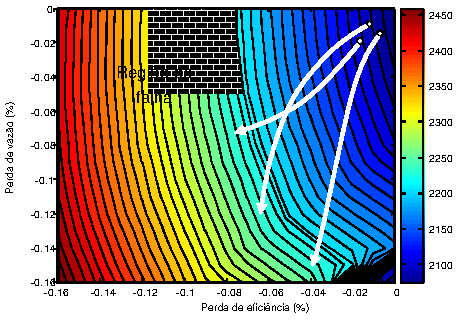
\includegraphics[width=\textwidth]{artigo_limite_falha}
      \scriptsize Cores: temperatura dos gases de escape (°R).
    \end{column}
    \begin{column}{0.50\textwidth}
      \begin{itemize}
        \item O simulador acompanha limites como \textbf{temperatura máxima} e \textbf{estabilidade do fluxo de ar} nos compressores.
        \item A \textbf{margem operacional} indica quanto o motor ainda está afastado de cada limite.
        \item Ao atingir qualquer desses limites, a trajetória termina. Esse é o ciclo de falha \textbf{$T$}, usado para calcular a RUL.
      \end{itemize}
    \end{column}
  \end{columns}
  \fonte{As linhas mostram trajetórias de degradação nos eixos de perda de eficiência e de vazão. ``Falha'' é atingir um limite do cenário simulado; não significa necessariamente ruptura física. Fonte: Saxena et al. (2008), seção V.D e fig. 8, pp. 6--7.}
  \note{Explique primeiro os eixos: os caminhos mostram perdas de eficiência e de capacidade de vazão. O término indica atingir um limite operacional do simulador, não uma ruptura física catastrófica. As margens incluem temperatura e margem de estol do fan e dos compressores. O símbolo I_sim distingue esse índice da margem H usada mais adiante para ajustar a previsão. A temperatura interna EGT é T48 na saída da HPT; T50 é uma medição diferente, na saída da LPT.}
\end{frame}

\begin{frame}{Índice de saúde: como ler a equação}
  O índice de saúde acompanha a \textbf{menor margem operacional} do motor:
  \[
    I_{\mathrm{sim}}(t)=\min_j m_j(t).
  \]
  \begin{itemize}
    \item $t$: ciclo de operação; $j$: identifica cada limite acompanhado.
    \item $m_j(t)$: margem até o limite $j$, convertida para uma escala comum entre 0 e 1. Essa conversão é a \textbf{normalização}.
    \item $\min_j$: escolha a menor margem entre todos os limites.
    \item $I_{\mathrm{sim}}(t)$: índice de saúde interno ao simulador, naquele ciclo.
  \end{itemize}
  \begin{block}{A escala das margens}
    \textbf{1}: condição saudável de referência.\qquad \textbf{0}: limite atingido.\\
    Temperatura e estabilidade do fluxo passam a ter margens comparáveis.
  \end{block}
  \fonte{Síntese da definição de Saxena et al. (2008), seção V.D, pp. 6--7. Quanto menor a margem normalizada, mais próximo está o respectivo limite nessa escala.}
  \note{Leia a equação em voz alta como uma instrução: no ciclo atual, calcule as margens na mesma escala e escolha a menor. A normalização evita comparar diretamente valores com unidades e limites físicos diferentes.}
\end{frame}

\begin{frame}{Por que escolher a menor margem?}
  \textbf{Exemplo didático:} três margens já convertidas para a escala de 0 a 1.
  \par\medskip
  \begin{center}
    \begin{tabular}{@{}lc@{}}
      \toprule
      Limite acompanhado & Margem normalizada \\
      \midrule
      Temperatura dos gases & \textbf{0,20} \\
      Estabilidade do fluxo no compressor & 0,65 \\
      Estabilidade do fluxo no fan & 0,80 \\
      \bottomrule
    \end{tabular}
  \end{center}
  \[
    I_{\mathrm{sim}}(t)=\min\{0{,}20;\;0{,}65;\;0{,}80\}=\mathbf{0{,}20}.
  \]
  \begin{itemize}
    \item Neste exemplo, a temperatura determina o índice de saúde.
    \item Usar a média esconderia a menor margem: margens maiores nos outros limites \textbf{não compensam} a condição crítica.
    \item \textbf{Uma margem em zero} leva o índice a zero e encerra a trajetória.
  \end{itemize}
  \fonte{Valores ilustrativos. A regra do mínimo corresponde ao critério de término descrito por Saxena et al. (2008), seção V.D.}
\end{frame}

\begin{frame}{Índice de saúde e RUL respondem a perguntas diferentes}
  \begin{columns}[T]
    \begin{column}{0.47\textwidth}
      \textbf{Índice de saúde: condição atual}
      \begin{itemize}
        \item Quanto resta da margem operacional mais crítica?
        \item Usa uma escala sem unidade, de 0 a 1.
        \item $I_{\mathrm{sim}}=0{,}20$ descreve a margem normalizada atual.
      \end{itemize}
    \end{column}
    \begin{column}{0.47\textwidth}
      \textbf{RUL: tempo restante}
      \begin{itemize}
        \item Quantos ciclos faltam até atingir o limite?
        \item É expressa em ciclos de operação.
        \item Depende também de como a degradação evolui ao longo do tempo.
      \end{itemize}
    \end{column}
  \end{columns}
  \medskip
  \begin{alertblock}{0,20 de índice de saúde não significa 20\,\% de vida restante}
    Dois motores podem ter o mesmo índice hoje e velocidades de degradação diferentes; por isso, podem ter RUL diferentes.
  \end{alertblock}
  \fonte{O índice interno do simulador não é fornecido explicitamente nos arquivos C-MAPSS. O modelo aprende a prever RUL a partir dos sensores. Fonte: Saxena et al. (2008), seções V.D e VI.}
  \note{Distinga também este índice interno do indicador de saúde construído a partir dos sensores, apresentado mais adiante como uma alternativa de detecção. Eles têm origens e funções diferentes.}
\end{frame}

\begin{frame}{Estrutura dos arquivos}
      Cada linha é um ciclo de um motor, com 26 colunas:
      \begin{itemize}
        \item identificador do motor e número do ciclo;
        \item 3 ajustes operacionais;
        \item 21 sensores.
      \end{itemize}
      \medskip
      Três arquivos por subconjunto:
      \begin{itemize}
        \item \texttt{train\_FD00x}: trajetórias \textbf{até a falha};
        \item \texttt{test\_FD00x}: trajetórias \textbf{interrompidas} antes da falha;
        \item \texttt{RUL\_FD00x}: vida remanescente verdadeira no último ciclo de cada motor de teste.
      \end{itemize}
  \fonte{``Trajetória'' é a sequência de registros de um motor ao longo dos ciclos. ``Truncada'' significa que os registros terminam antes da falha.}
\end{frame}

\begin{frame}{RUL: quantos ciclos ainda restam?}
      A vida remanescente verdadeira é o ciclo da falha menos o ciclo atual:
      \[
        \RUL(t) = T - t.
      \]
      $T$: ciclo da falha.\quad $t$: ciclo atual.
      \begin{block}{Exemplo didático}
        Se o motor falha no ciclo 200, no ciclo 160 restam $200-160=40$ ciclos.
      \end{block}
      \medskip
      \textbf{Rótulo de treino:} o valor que o modelo aprende a prever.
      Uma convenção é limitar esse valor a 125 ciclos:
      \[
        \RUL_{125}(t) = \min\{T - t,\,125\}.
      \]
      Se faltam 180 ciclos, o rótulo com teto vale 125; se faltam 40, vale 40.
      \fonte{O teto simplifica o alvo de aprendizado. Ele não identifica o início físico da degradação, que deve ser estimado a partir das medições.}
  \note{T é conhecido nas trajetórias completas usadas para avaliar o modelo. Durante a operação, temos as leituras até t e uma previsão de RUL; o ciclo futuro de falha permanece desconhecido.}
\end{frame}

\begin{frame}{Os 21 sensores}
  \footnotesize
  \begin{columns}[T]
    \begin{column}{0.49\textwidth}
      \begin{tabular}{@{}rll@{}}
        \toprule
        \# & Símbolo & Descrição \\
        \midrule
        1 & T2 & Temperatura: entrada do fan \\
        2 & \textbf{T24} & Temperatura: saída do LPC \\
        3 & \textbf{T30} & Temperatura: saída do HPC \\
        4 & \textbf{T50} & Temperatura: saída da LPT \\
        5 & P2 & Pressão: entrada do fan \\
        6 & P15 & Pressão: duto de \emph{bypass} \\
        7 & \textbf{P30} & Pressão total: saída do HPC \\
        8 & \textbf{Nf} & Rotação física do fan \\
        9 & \textbf{Nc} & Rotação física do núcleo \\
        10 & epr & Razão de pressão do motor \\
        11 & \textbf{Ps30} & Pressão estática: saída do HPC \\
        \bottomrule
      \end{tabular}
    \end{column}
    \begin{column}{0.49\textwidth}
      \begin{tabular}{@{}rll@{}}
        \toprule
        \# & Símbolo & Descrição \\
        \midrule
        12 & \textbf{phi} & Vazão de combustível / Ps30 \\
        13 & \textbf{NRf} & Rotação corrigida do fan \\
        14 & \textbf{NRc} & Rotação corrigida do núcleo \\
        15 & BPR & Razão de \emph{bypass} \\
        16 & farB & Razão combustível/ar \\
        17 & \textbf{htBleed} & Entalpia de sangria \\
        18 & Nf\_dmd & Rotação demandada do fan \\
        19 & PCNfR\_dmd & Rotação corrigida demandada \\
        20 & \textbf{W31} & Ar de arrefecimento: HPT \\
        21 & \textbf{W32} & Ar de arrefecimento: LPT \\
        \bottomrule
      \end{tabular}
    \end{column}
  \end{columns}
  \smallskip
  \footnotesize
  Em negrito, os 13 sensores usados no estudo. BPR varia no FD001 e foi excluído por decisão de projeto; os demais canais não destacados são constantes ou quase constantes.
  \fonte{Unidades originais: °R = graus Rankine; psia = libras por polegada quadrada, pressão absoluta; rpm = rotações por minuto; lbm/s = libras de massa por segundo. Fonte: Saxena et al. (2008), tabela 2.}
\end{frame}

\begin{frame}{Como ler os nomes dos sensores}
  \begin{itemize}
    \item \textbf{Rotação:} velocidade de giro. A rotação corrigida considera as condições do ar na entrada, para permitir comparações.
    \item \textbf{Vazão:} quantidade de fluido que passa por unidade de tempo. W31/W32 medem ar usado para \textbf{arrefecimento}, isto é, resfriamento.
    \item \textbf{BPR:} razão entre a vazão de ar pelo bypass e a vazão pelo núcleo.
    \item \textbf{Sangria:} retirada de parte do ar comprimido. A entalpia descreve o conteúdo energético desse ar.
    \item \textbf{Pressão estática e total:} a primeira descreve a pressão local; a segunda também considera o efeito do movimento do ar.
  \end{itemize}
  \fonte{Glossário para a tabela anterior. Os símbolos e as unidades originais são mantidos para facilitar a leitura dos arquivos C-MAPSS.}
  \note{Retome apenas os termos necessários para interpretar os gráficos. Os alunos não precisam memorizar a lista dos 21 sensores para compreender a decisão de manutenção.}
\end{frame}

\begin{frame}{Como a degradação aparece nos sensores}
  \centering
  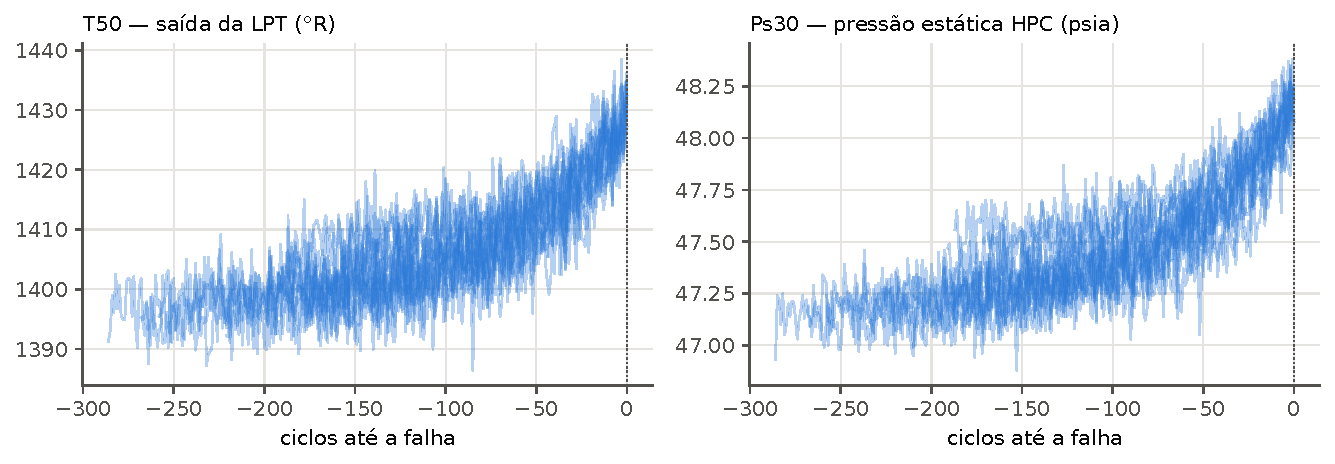
\includegraphics[width=0.95\textwidth]{sensores_fd001}
  \vfill
  \begin{itemize}
    \item No eixo horizontal, 0 é a falha; $-100$ indica 100 ciclos antes dela.
    \item As curvas de 12 motores do FD001 mostram oscilações e aumento perto da falha.
    \item Compare cada motor com seu nível inicial: a \textbf{linha de base do motor}.
  \end{itemize}
  \note{O alinhamento pelo ciclo final é uma visualização retrospectiva. Em operação, o ciclo de falha ainda é desconhecido; o detector precisa usar as medições disponíveis até o ciclo atual.}
\end{frame}

\begin{frame}{Uma melhora momentânea pode ocorrer durante a degradação}
  \centering
  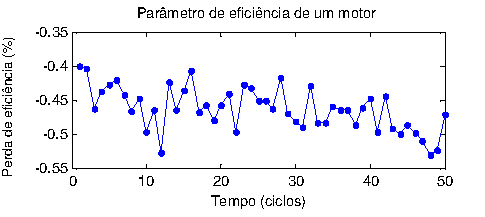
\includegraphics[height=3.2cm]{artigo_oscilacoes}
  \medskip
  \begin{itemize}
    \item A tendência de desgaste convive com \textbf{oscilações locais}.
    \item Examine a sequência de observações para distinguir uma variação momentânea de uma mudança persistente.
    \item A suavização ajuda a ler a tendência; uma janela maior também pode \textbf{atrasar a detecção}.
  \end{itemize}
  \fonte{Adaptado de Saxena et al. (2008), fig. 5, p. 5. O gráfico mostra um parâmetro interno simulado, não um sensor disponível nos arquivos.}
  \note{O artigo incorpora efeitos simplificados de manutenção entre voos ao ruído de processo. Isso permite melhoras locais, mas não fornece um histórico explícito de intervenções ou trocas de módulo. A figura justifica examinar tendências; o tamanho da janela precisa ser escolhido e avaliado no experimento.}
\end{frame}

\begin{frame}{A vida útil varia muito entre motores}
  \centering
  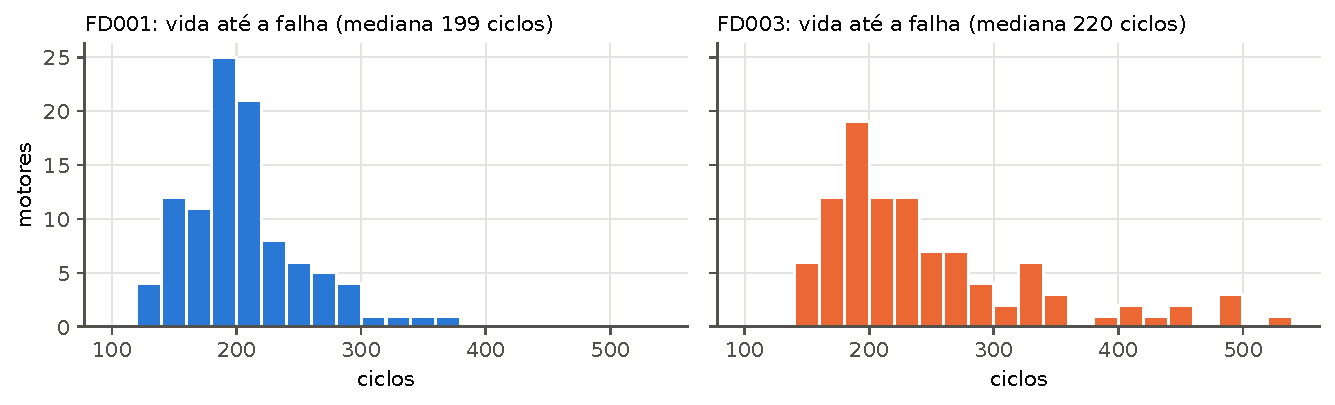
\includegraphics[width=\textwidth]{vida_histograma}
  \vfill
  No FD001, a vida vai de 128 a 362 ciclos. Uma regra única de remoção por idade, igual para toda a frota, ou remove cedo demais a maioria dos motores ou deixa alguns falharem. Esse é o argumento econômico do monitoramento de condição.
\end{frame}

%=====================================================================
\section{O problema de decisão}

\begin{frame}{A curva P--F}
  \centering
  \begin{tikzpicture}[x=0.95cm,y=0.70cm,>=Stealth]
    \draw[->,tinta2] (0,0) -- (12.5,0) node[below left,font=\footnotesize]{tempo (ciclos)};
    \draw[->,tinta2] (0,0) -- (0,4.4) node[above right,font=\footnotesize]{condição do motor};
    \draw[very thick,serieA] (0.2,3.6) -- (4,3.55) .. controls (6.5,3.4) and (8.5,2.4) .. (9.8,0.3);
    \fill[serieB] (4.4,3.52) circle (2.5pt);
    \node[font=\footnotesize,anchor=south] at (4.4,3.7) {\textbf{P}: falha potencial detectável};
    \fill[black] (9.8,0.3) circle (2.5pt);
    \node[font=\footnotesize,anchor=west] at (10.0,0.35) {\textbf{F}: falha funcional};
    \draw[dashed,serieC,thick] (6.6,0) -- (6.6,3.2);
    \draw[dashed,serieC,thick] (8.9,0) -- (8.9,1.6);
    \draw[<->,serieC] (6.6,2.2) -- (8.9,2.2) node[midway,above,font=\footnotesize]{$L$};
    \node[serieC,font=\footnotesize,anchor=north] at (6.6,-0.05) {alarme $t_a$};
    \node[serieC,font=\footnotesize,anchor=north] at (8.9,-0.05) {remoção $t_a{+}L$};
    \draw[decorate,decoration={brace,amplitude=5pt,mirror},tinta2] (4.4,-0.75) -- (9.8,-0.75)
      node[midway,below=6pt,font=\footnotesize]{intervalo P--F: janela para planejar};
  \end{tikzpicture}
  \vspace{-2mm}
  \begin{itemize}
    \item \textbf{P}: primeiro sinal detectável de degradação. \textbf{F}: falha funcional, quando o motor deixa de atender ao desempenho exigido.
    \item Após detectar P, precisamos de $L$ ciclos para preparar e executar a remoção: motor reserva, vaga de oficina, material e mão de obra. Esse é o \textbf{tempo logístico}.
  \end{itemize}
\end{frame}

\begin{frame}{Objetivo}
  \begin{block}{Pergunta}
    Em que ciclo emitir o alarme de remoção de cada motor, de modo que
    \begin{enumerate}
      \item a remoção aconteça \textbf{a tempo de evitar a falha funcional}, e
      \item a relação \textbf{receita de voar} / \textbf{despesa com manutenção de motores} seja a melhor possível no longo prazo?
    \end{enumerate}
  \end{block}
  \medskip
  \begin{columns}[T]
    \begin{column}{0.48\textwidth}
      \textbf{Remover tarde} (depois de F)
      \begin{itemize}
        \item remoção não programada, custo $c_f$;
        \item impacto em disponibilidade e segurança.
      \end{itemize}
    \end{column}
    \begin{column}{0.48\textwidth}
      \textbf{Remover cedo}
      \begin{itemize}
        \item custo planejado $c_p < c_f$;
        \item mas vida útil desperdiçada: menos ciclos de receita por remoção, mais remoções ao longo dos anos.
      \end{itemize}
    \end{column}
  \end{columns}
\end{frame}

\begin{frame}{Receita \emph{versus} despesa no longo prazo}
  Distribua o custo de manutenção pelos ciclos voados: remover cedo demais pode aumentar o custo por ciclo.
  \medskip
  \begin{center}
    \begin{tabular}{@{}lrr@{}}
      \toprule
      Exemplo didático & Custo & Ciclos voados \\
      \midrule
      Remoção planejada A & 1 & 100 \\
      Remoção planejada B & 1 & 200 \\
      \bottomrule
    \end{tabular}
  \end{center}
  \begin{itemize}
    \item A: $1/100=0{,}010$ unidade de custo por ciclo.
    \item B: $1/200=0{,}005$ unidade de custo por ciclo.
    \item Com o mesmo custo de remoção, aproveitar mais ciclos reduz o custo por ciclo. A remoção precisa ocorrer a tempo.
  \end{itemize}
  \fonte{Valores ilustrativos. A avaliação da frota soma os custos e divide pela soma dos ciclos; inclui remoções planejadas e após falha.}
  \note{Comece pela divisão custo/ciclos. Depois apresente o formalismo do slide seguinte, que expressa a mesma ideia no longo prazo.}
\end{frame}

\begin{frame}{A mesma ideia em uma fórmula}
  Instalar outro motor inicia um novo período: \textbf{renovação com recompensa}.
  \begin{itemize}
    \item $U$: ciclos voados; $C$: custo da remoção ($c_p$ planejada, $c_f$ após F).
    \item $r$: receita líquida por ciclo, antes da manutenção do motor.
    \item $\mathbb{E}[U]$ e $\mathbb{E}[C]$: médias esperadas de ciclos e custos.
  \end{itemize}
  No longo prazo, pelo teorema da renovação com recompensa:
  \[
    g=\frac{\mathbb{E}[C]}{\mathbb{E}[U]},\qquad
    \frac{\text{lucro}}{\text{ciclo}}=r-g,\qquad
    \frac{\text{receita}}{\text{despesa}}=\frac{r}{g}.
  \]
  Para receita $r$ fixa, \textbf{minimizar o custo por ciclo $g$} maximiza o lucro por ciclo e a relação receita/despesa. A remoção deve ocorrer antes de F.
  \par\smallskip
  Com $n$ motores: $\hat g = \sum_i C_i \,/\, \sum_i U_i$ (custo total / ciclos totais).
  \fonte{Usamos o custo planejado como unidade: $c_p=1$. A razão $R=c_f/c_p$ indica quantas vezes uma falha custa mais que uma remoção planejada.}
\end{frame}

\begin{frame}{Referência simples: remover por idade}
  \begin{columns}[c]
    \begin{column}{0.58\textwidth}
      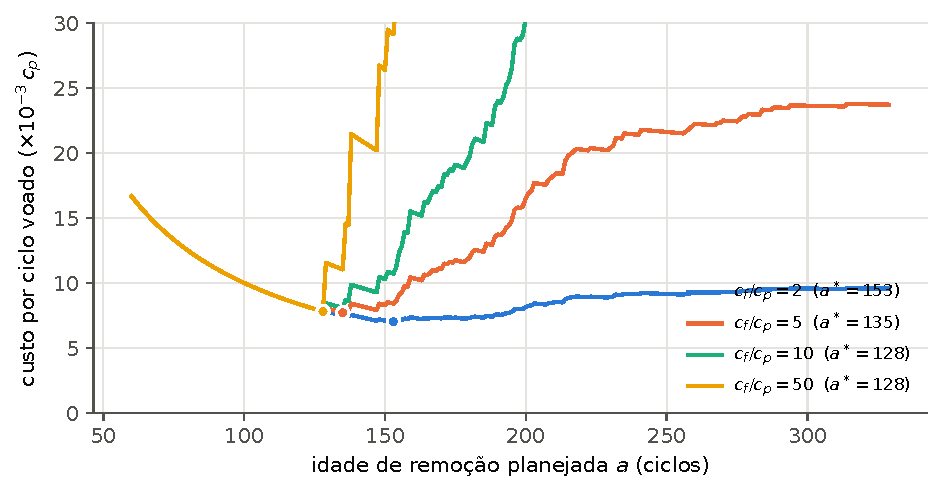
\includegraphics[width=\textwidth]{custo_idade}
    \end{column}
    \begin{column}{0.40\textwidth}
      Remover todo motor na idade $a$, sem olhar sensores:
      \begin{itemize}
        \item $a$ pequeno: poucas falhas, muita vida desperdiçada;
        \item $a$ grande: muitas falhas caras.
      \end{itemize}
      \medskip
      Neste conjunto, com falha cara ($R \geq 10$), a idade ótima cai para \textbf{128 ciclos}. Um motor com a vida mediana de 199 ciclos perderia $199-128=71$ ciclos de uso.
      \medskip

      \alert{O monitoramento de condição só vale a pena se superar esta referência.}
    \end{column}
  \end{columns}
\end{frame}

\begin{frame}{Erros iguais podem ter consequências diferentes}
  Considere um motor com \textbf{20 ciclos} de vida remanescente.
  \medskip
  \begin{columns}[c]
    \begin{column}{0.44\textwidth}
      \centering
      \begin{tikzpicture}[x=0.43cm,y=0.26cm,>=Stealth]
        \draw[->,tinta2] (-5.6,0) -- (5.8,0);
        \draw[->,tinta2] (0,0) -- (0,11.5);
        \draw[very thick,serieA] (-5,5) -- (0,0);
        \draw[very thick,serieB] (0,0) -- (5,10);
        \foreach \x in {-5,0,5}
          \node[below,font=\footnotesize] at (\x,0) {\x};
        \node[above left,font=\footnotesize] at (0,11.5) {Penalidade};
        \node[below,font=\footnotesize] at (0,-1.0) {Erro de RUL (ciclos)};
        \fill[serieA] (-5,5) circle (2pt);
        \fill[serieB] (5,10) circle (2pt);
        \node[above left,font=\footnotesize,serieA] at (-5,5) {5};
        \node[above right,font=\footnotesize,serieB] at (5,10) {10};
      \end{tikzpicture}
    \end{column}
    \begin{column}{0.53\textwidth}
      \begin{itemize}
        \item Prever \textbf{15 ciclos}: erro $-5$. A intervenção pode ser antecipada, com vida útil desperdiçada.
        \item Prever \textbf{25 ciclos}: erro $+5$. O planejador recebe um tempo que o motor não tem.
        \item O erro absoluto é igual; a \textbf{consequência operacional} muda.
      \end{itemize}
    \end{column}
  \end{columns}
  \fonte{Função ilustrativa redesenhada de Saxena et al. (2008), fig. 10, p. 8. Erro = RUL prevista $-$ RUL verdadeira.}
  \note{Peça que os alunos comparem as duas previsões antes de mostrar a penalidade. O gráfico simplificado atribui peso maior à superestimação. Ele expressa uma preferência entre erros; a avaliação econômica da aula usa custo por ciclo e as consequências da política de remoção.}
\end{frame}

\begin{frame}{O que a margem muda nas previsões?}
  \begin{columns}[c]
    \begin{column}{0.49\textwidth}
      \centering
      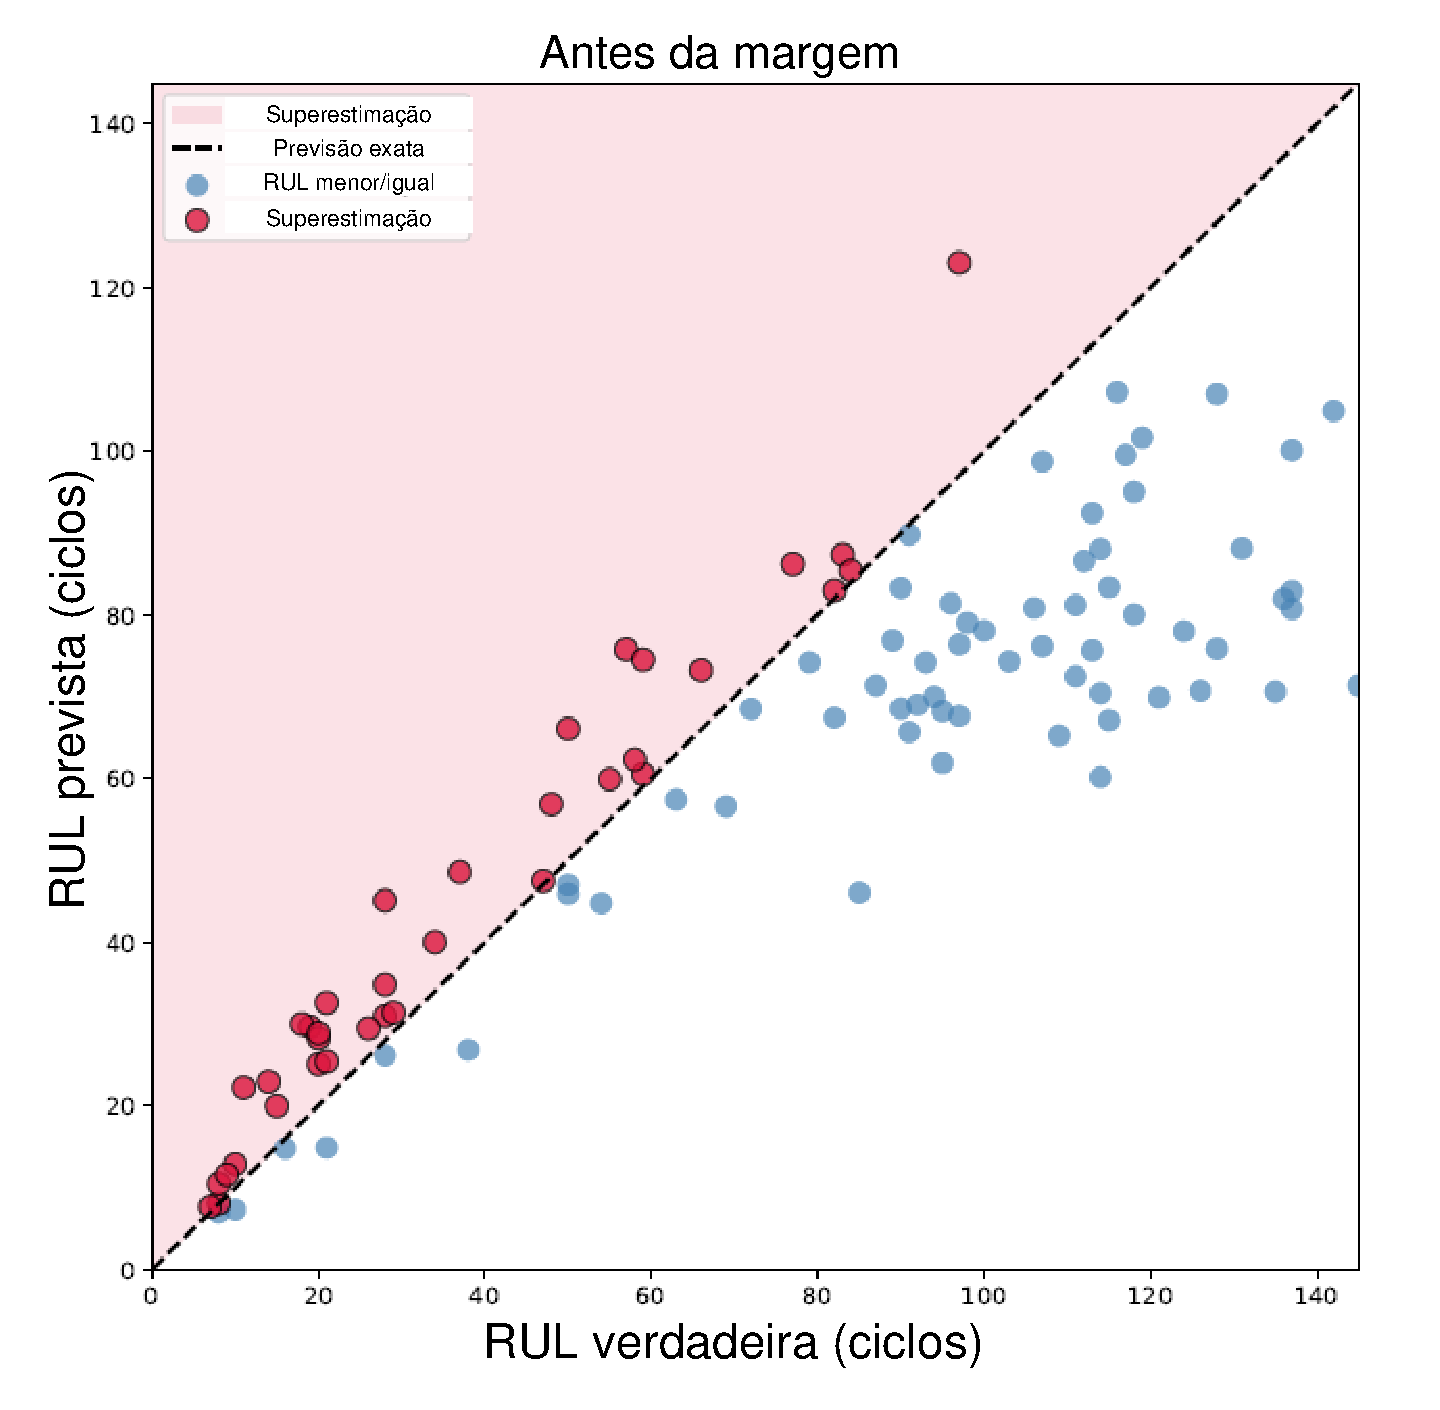
\includegraphics[height=4.7cm]{amanda_rul_antes}
    \end{column}
    \begin{column}{0.49\textwidth}
      \centering
      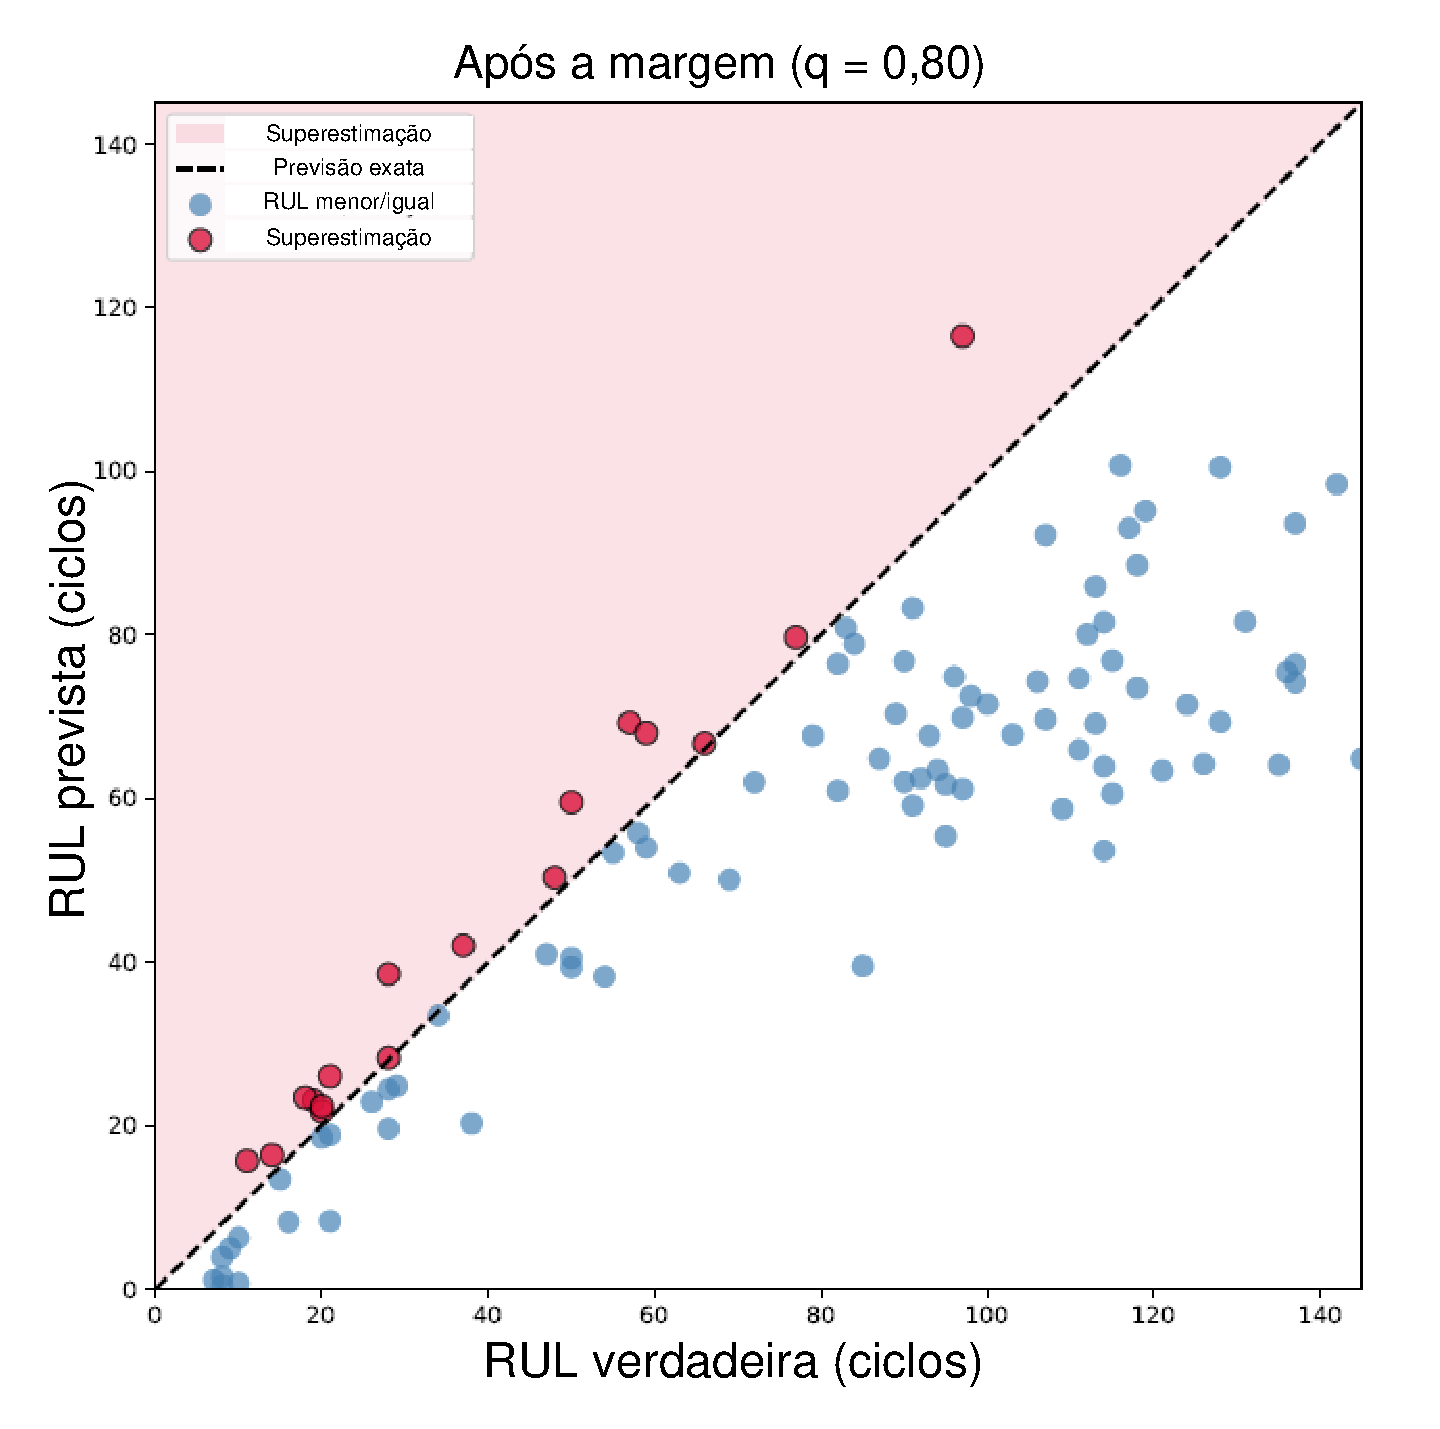
\includegraphics[height=4.7cm]{amanda_rul_depois}
    \end{column}
  \end{columns}
  \small
  \textbf{Diagonal:} previsão igual à RUL verdadeira.\quad
  \textbf{Acima:} superestimação.\\
  Subtrair a margem desloca as previsões para baixo e antecipa a ação.
  \fonte{Bassani (2026), slide 27: CatBoost, FD001, janela de 15 ciclos, teste oficial. Após correção: quantil 0,80, margem de 6,56 ciclos.}
  \note{Identifique os eixos antes de interpretar as cores. Os pontos vermelhos superestimam a vida remanescente. A margem reduz parte dessas ocorrências, mas também desloca previsões que já eram conservadoras. Estes resultados pertencem ao estudo de Amanda; os gráficos preliminares de LightGBM da aula vêm de outro protocolo.}
\end{frame}

\begin{frame}{Uma margem calculada a partir dos erros}
  Reserve motores para \textbf{calibração}: observe quanto a previsão excede a vida verdadeira.
  \par\medskip
  \centering
  \small
  \begin{tabular}{@{}lrrrrr@{}}
    \toprule
    Motor & 1 & 2 & 3 & 4 & 5 \\
    \midrule
    RUL prevista & 20 & 21 & 14 & 10 & 10 \\
    RUL verdadeira & 28 & 17 & 11 & 8 & 9 \\
    Erro: prevista $-$ verdadeira & $-8$ & 4 & 3 & 2 & 1 \\
    \midrule
    RUL após subtrair 3 ciclos & 17 & 18 & 11 & 7 & 7 \\
    \bottomrule
  \end{tabular}
  \par\medskip
  \raggedright
  Erros ordenados: $-8,\,1,\,2,\,3,\,4$. O percentil 75 é \textbf{3 ciclos}.
  \[
    H=\max\{Q_{0{,}75}(\RULhat-\RUL),0\},\qquad
    \RUL_{\mathrm{ajustada}}=\max\{\RULhat-H,0\}.
  \]
  \small
  $Q_{0{,}75}$ marca o corte de 75\,\% na distribuição dos erros; $\max\{\cdot,0\}$ fixa o mínimo em zero.\\
  No motor 2, a previsão cai de 21 para 18 ciclos; a vida verdadeira é 17.
  \fonte{Exemplo didático adaptado de Bassani (2026), slides 21--23. Todas as vidas e os erros estão em ciclos.}
  \note{Explique quantil como um ponto de corte na lista de erros ordenados. O exemplo usa cinco posições para tornar a conta visível. A margem reduz a superestimação do motor 2, mas ainda resta um ciclo de excesso. Fixe a margem nos dados de desenvolvimento e avalie em motores separados. Um percentil dos erros não garante a mesma proporção de remoções antes da falha numa política sequencial.}
\end{frame}

\begin{frame}{Quando emitir o alarme? Um exemplo}
  A remoção exige antecedência para conseguir motor reserva, equipe e recursos.
  \begin{description}[Tempo logístico]
    \item[Tempo logístico] $L=20$ ciclos entre o alarme e a remoção.
    \item[Previsão de RUL] 25 ciclos de vida remanescente no ciclo atual, $t=150$.
    \item[Margem] Subtraímos $H=5$ ciclos: a previsão ajustada é $25-5=20$.
  \end{description}
  \begin{block}{Decisão neste ciclo}
    A previsão ajustada chegou ao tempo necessário para agir: \textbf{emitimos o alarme no ciclo 150}. A remoção fica programada para $150+20=170$.
  \end{block}
  \fonte{Exemplo didático após a detecção de P. A previsão pode errar; a margem antecipa a ação, mas não garante uma remoção antes da falha.}
  \note{Pergunte: se a RUL ajustada ainda fosse 30 ciclos, o que faria a regra? Ela continuaria monitorando. O alarme é emitido no primeiro ciclo em que a RUL ajustada fica menor ou igual a L.}
\end{frame}

\begin{frame}{Regra de decisão com tempo logístico}
  Alarme: \textbf{primeiro ciclo} em que a previsão ajustada chega ao tempo logístico.
  Use somente os dados disponíveis até o ciclo atual $t$:
  \[
    \text{alarme em } t_a = \min\{\, t \geq t_P : \RULhat(t) - H \leq L \,\}
  \]
  \begin{itemize}
    \item $t_P$: ciclo em que o ponto P foi detectado (ou $t_P = 1$ numa política sem detecção);
    \item $\RULhat(t)$: vida remanescente prevista;
    \item $H$: \textbf{margem de segurança}, escolhida para minimizar $g$;
    \item $L$: tempo logístico; $t_a$: ciclo do alarme; remoção em $t_a + L$.
  \end{itemize}
  \smallskip
  \begin{columns}[T]
    \begin{column}{0.48\textwidth}
      \textbf{Planejamento perdido:} $t_a + L > T$. O motor falha antes da remoção (ou nunca houve alarme).
    \end{column}
    \begin{column}{0.48\textwidth}
      \textbf{Vida desperdiçada:} $T - (t_a + L)$, nas remoções planejadas.
    \end{column}
  \end{columns}
  \fonte{Na simulação, remoção até o ciclo $T$ conta como planejada; depois de $T$, como falha. $H$ é escolhido por custo nos motores usados para desenvolver a regra.}
  \note{Retome o exemplo anterior para distinguir duas escolhas: uma margem baseada em quantis e uma margem escolhida pelo custo da política. Em ambas, a avaliação final deve usar motores que não participaram da escolha. L representa a antecedência necessária para conseguir recursos e executar a intervenção.}
\end{frame}

%=====================================================================
\section{Abordagem}

\begin{frame}{Dois estágios para apoiar a decisão}
  \centering
  \begin{tikzpicture}[node distance=6mm and 4mm, box/.style={draw=tinta2,rounded corners,align=center,minimum height=12mm,text width=20mm,font=\footnotesize}]
    \node[box] (s) {21 sensores\\por ciclo};
    \node[box,right=of s] (m) {Média móvel\\(25 ciclos)};
    \node[box,right=of m,draw=serieB,thick] (p) {\textbf{1. Detectar P}\\desvio da linha\\de base do motor};
    \node[box,right=of p,draw=serieA,thick] (r) {\textbf{2. Prever RUL}\\após P\\(LightGBM)};
    \node[box,right=of r,draw=serieC,thick] (a) {\textbf{Decisão}\\emitir alarme\\$\RULhat - H \leq L$};
    \draw[->,thick,tinta2] (s) -- (m);
    \draw[->,thick,tinta2] (m) -- (p);
    \draw[->,thick,tinta2] (p) -- (r);
    \draw[->,thick,tinta2] (r) -- (a);
    \node[below=4mm of p,font=\footnotesize,text width=30mm,align=center] {sem P: monitoramento normal};
  \end{tikzpicture}
  \vfill
  \begin{itemize}
    \item O estágio 1 identifica um desvio da condição inicial; o estágio 2 prevê a vida remanescente após essa detecção.
    \item \textbf{Média móvel:} média das leituras mais recentes; reduz oscilações e ajuda a observar a tendência.
    \item No ciclo $t$, o processamento usa \textbf{somente medições disponíveis até $t$}.
  \end{itemize}
  \fonte{LightGBM é o modelo de aprendizado usado para prever RUL. A linha de base resume as primeiras leituras de cada motor.}
\end{frame}

\begin{frame}{O que o modelo recebe de cada janela?}
  Uma \textbf{janela} reúne ciclos recentes. Dela extraímos resumos, chamados de \textbf{atributos}, para descrever o sinal de cada sensor.
  \medskip
  \begin{description}[Assimetria]
    \item[Média] Nível médio do sinal na janela.
    \item[Variância] Quanto os valores se espalham ao redor da média.
    \item[Assimetria] Se a distribuição se estende mais para valores altos ou baixos.
    \item[RMS] Raiz da média dos quadrados: resume a magnitude dos valores.
  \end{description}
  \fonte{Nesta arquitetura, os atributos são calculados a partir da média móvel de cada sensor. RMS = \emph{Root Mean Square}. As janelas usam somente ciclos já observados.}
  \note{Uma mudança persistente pode alterar o nível, a dispersão ou a forma da distribuição. Atributos são números que descrevem esses aspectos e alimentam o modelo preditivo.}
\end{frame}

\begin{frame}{P detectado: um exemplo em um único sensor}
  \centering
  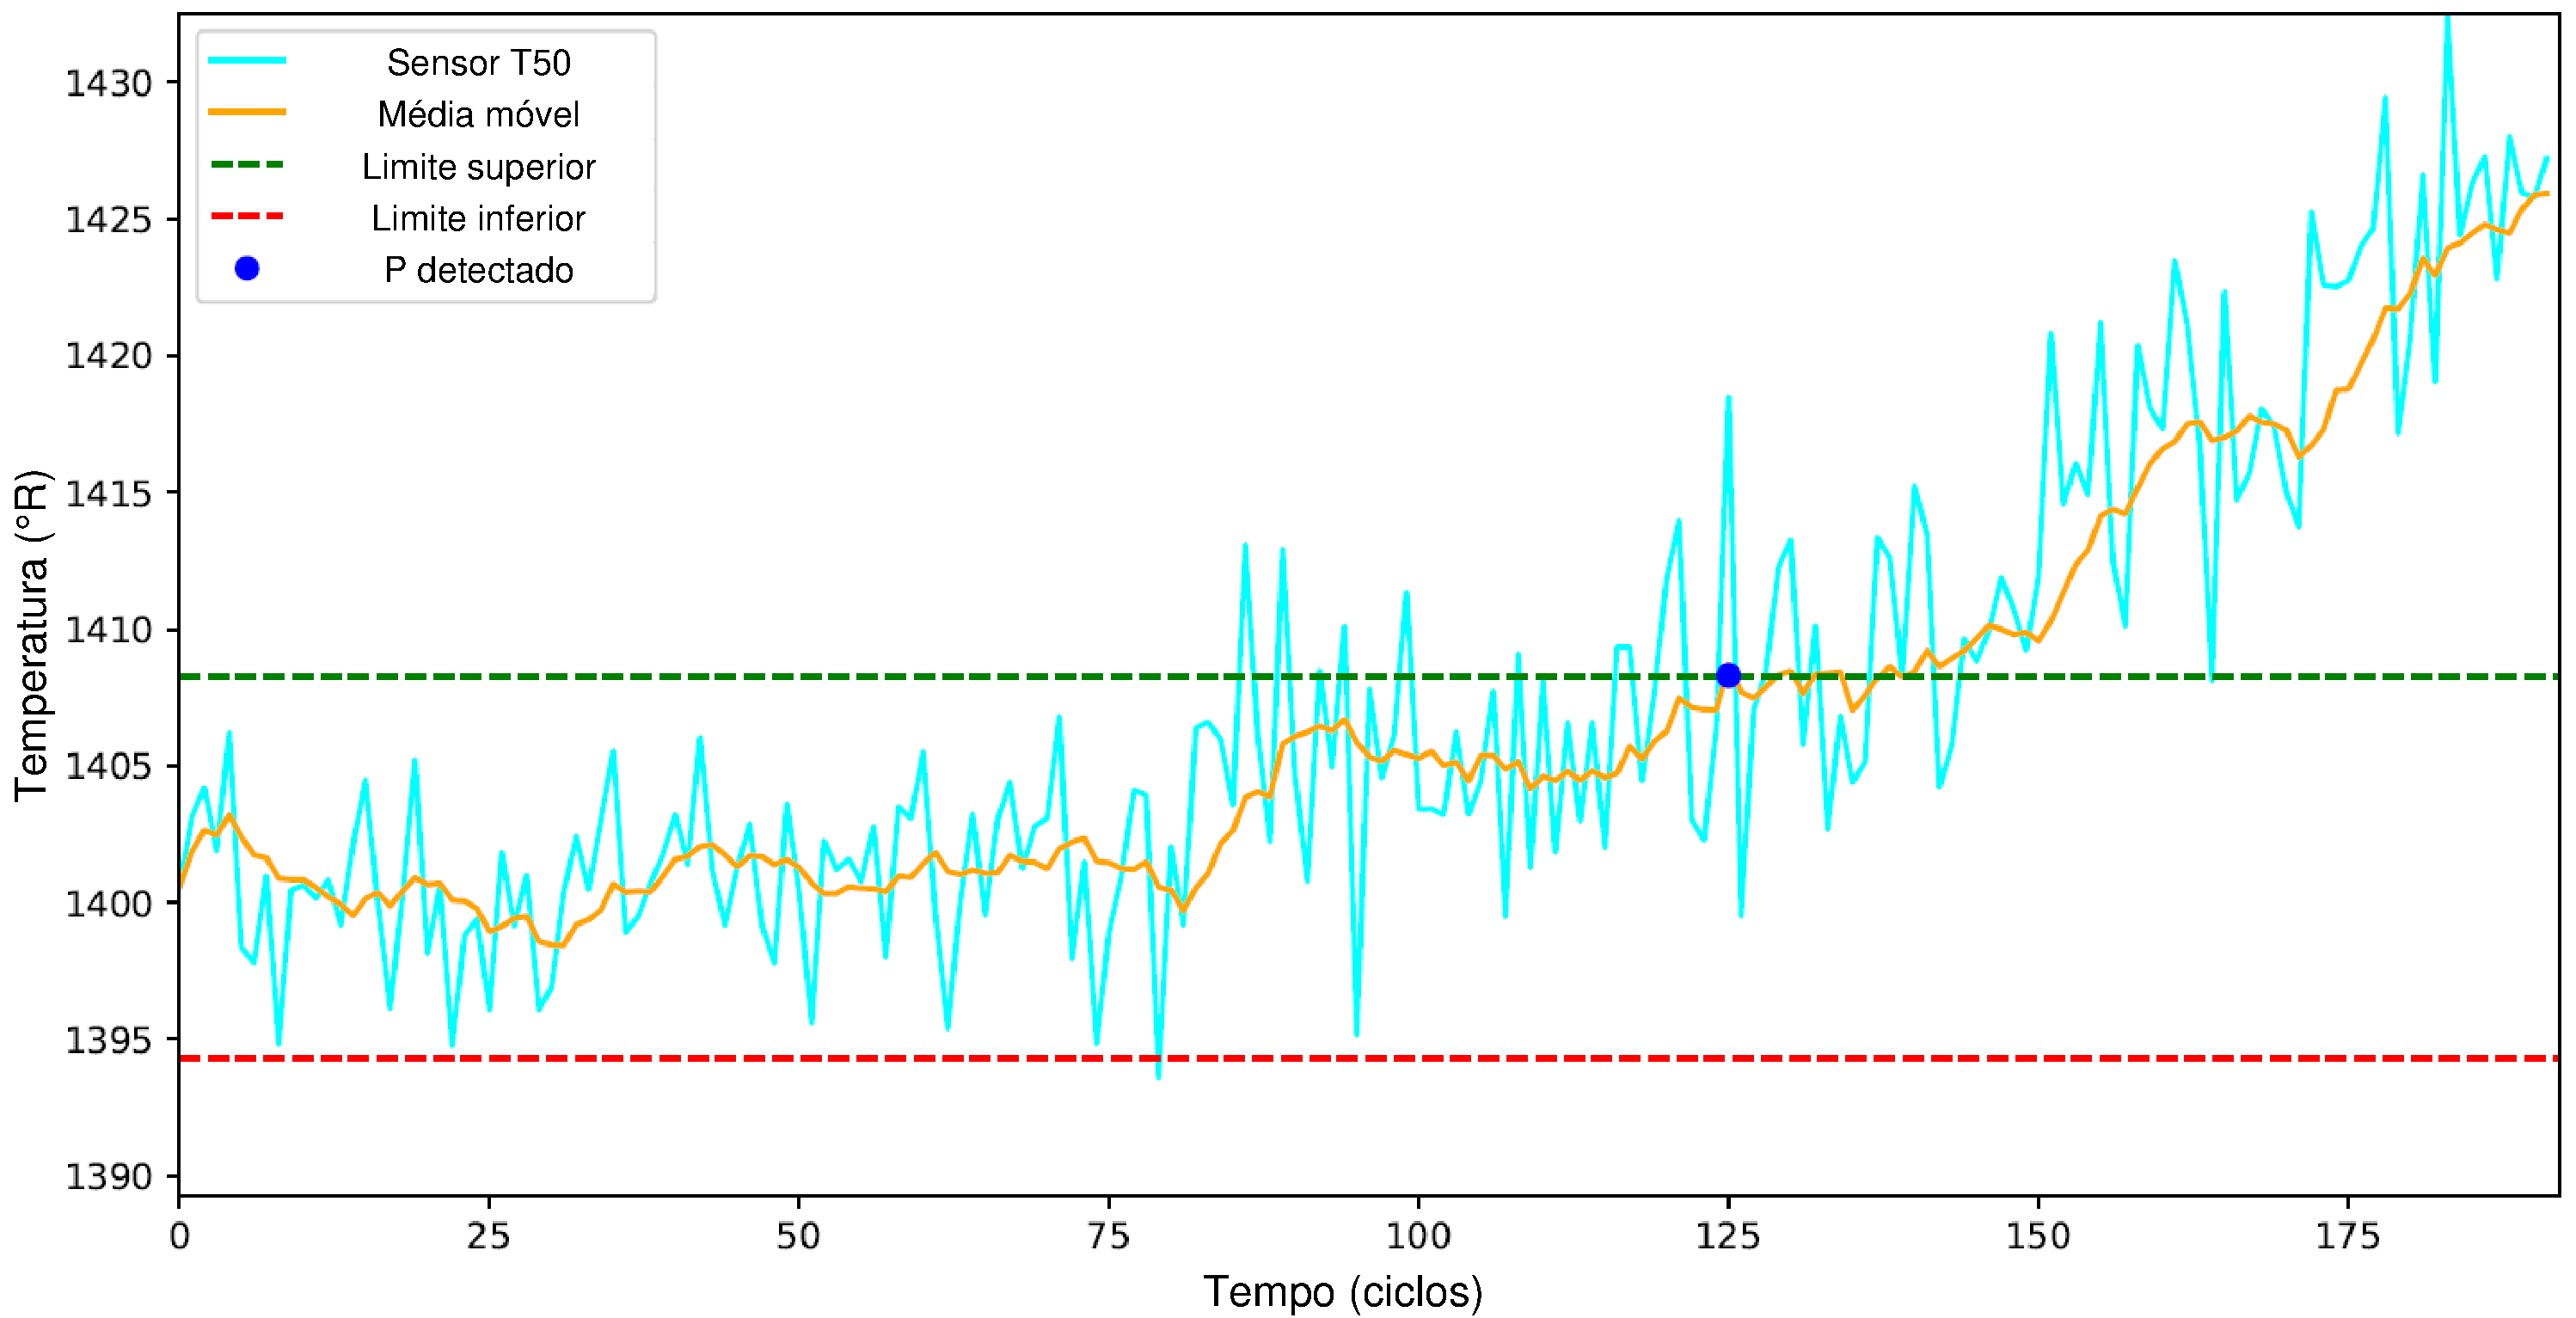
\includegraphics[height=4.9cm]{amanda_deteccao_p}
  \par
  \small
  A média móvel cruza o limite superior por volta do ciclo 125.
  Esse é o \textbf{ponto detectado pela regra}, estimado a partir das leituras.
  \fonte{Bassani (2026), slide 16. Exemplo de T50: linha de base de 15 ciclos, média móvel de 15 ciclos e limites relativos de $\pm0{,}5\,\%$.}
  \note{Mostre primeiro o sinal azul claro, depois a média móvel laranja e os limites. A detecção ocorre quando a regra identifica o desvio; o início físico da degradação pode ser anterior. A janela deste gráfico é de 15 ciclos, como na defesa. Na arquitetura de LightGBM apresentada nesta aula, a média móvel usa 25 ciclos.}
\end{frame}

\begin{frame}{Como detectar o ponto P: a ideia}
  Compare a leitura suavizada com a \textbf{linha de base}: o nível médio dos primeiros 15 ciclos daquele motor.
  \medskip
  \begin{itemize}
    \item \textbf{Regra relativa:} sinaliza uma mudança maior que uma porcentagem fixa do nível inicial.
    \item \textbf{Limiar estatístico:} compara a mudança com o ruído habitual do sensor, considerando a média móvel.
    \item \textbf{Indicador de saúde:} combina sensores em um único número e acompanha sua mudança.
  \end{itemize}
  \begin{block}{Exemplo de uma mudança de 0,5\,\%}
    Em T50, com nível 1\,400\,°R, corresponde a 7\,°R. Em Ps30, com nível 47\,psia, corresponde a 0,235\,psia. Para comparar, precisamos considerar o ruído de cada sensor.
  \end{block}
  \fonte{Limiar é o valor de corte que aciona a detecção. Os valores do exemplo são aproximados.}
  \note{A mesma porcentagem do nível não representa a mesma raridade estatística em sensores com ruídos diferentes. Primeiro estabeleça essa ideia; depois apresente as expressões formais.}
\end{frame}

\begin{frame}{Como detectar o ponto P: as regras}
  Linha de base do motor $u$: média $\mu_{u,s}$ do sensor $s$ nos $B = 15$ primeiros ciclos.
  \medskip
  \begin{description}[Indicador de saúde]
    \item[Regra relativa] detectar P se algum sensor tiver
      $\bigl|\bar x_{u,s}(t) - \mu_{u,s}\bigr| > \delta\,\mu_{u,s}$, com $\delta = 0{,}5\,\%$ do \emph{nível} do sinal.
    \item[Limiar estatístico] detectar P se algum sensor tiver
      $\dfrac{\bigl|\bar x_{u,s}(t) - \mu_{u,s}\bigr|}{\sigma_s/\sqrt{n_t}} > k$,
      com $\sigma_s$ o ruído na linha de base e $n_t$ os ciclos da média móvel.
    \item[Indicador de saúde] combinação linear dos sensores ajustada para acompanhar a fração de vida $t/T$, com o mesmo limiar $k\sigma$.
  \end{description}
  \medskip
  \fonte{$u$: motor; $s$: sensor; $\bar x$: média móvel; $\mu$: nível inicial; $\sigma$: medida do ruído; $n_t$: ciclos na média; $k$: multiplicador do limiar. $T$ é usado para ajustar o indicador no treino; na aplicação, usam-se apenas os sensores disponíveis.}
\end{frame}

\begin{frame}{Políticas comparadas e referências ideais}
  \small \textbf{Política:} regra para decidir quando agir. \textbf{Oráculo:} referência hipotética com informação perfeita sobre a falha futura.
  \par\medskip
  \centering
  \small
  \begin{tabular}{@{}lll@{}}
    \toprule
    Política & Usa sensores? & Parâmetro ajustado \\
    \midrule
    Substituição por idade & não & idade $a$ \\
    Limiar sobre o indicador de saúde & sim, sem RUL & limiar do indicador \\
    RUL em estágio único (sem teto / teto 125) & sim & margem $H$ \\
    RUL em dois estágios & sim & margem $H$ \\
    \midrule
    \textbf{Oráculo após a detecção} & conhece RUL após P & --- \\
    \textbf{Oráculo total} & conhece $T$ & --- \\
    \bottomrule
  \end{tabular}
  \vfill
  \raggedright
  O \textbf{oráculo após P} revela a vida restante somente quando o detector sinaliza.
  O \textbf{oráculo total} conhece o ciclo da falha desde o início.
  \fonte{Essas referências ajudam a separar duas causas de atraso: detectar tarde e prever mal a vida restante. Elas não estão disponíveis na operação real.}
\end{frame}

\begin{frame}{Detectamos tarde ou previmos mal?}
  Compare a \textbf{porcentagem de motores com planejamento perdido}, indicada por $p$.
  \medskip
  \begin{center}
    \begin{tabular}{@{}lc@{}}
      \toprule
      Exemplo didático & Planejamento perdido \\
      \midrule
      Política com previsão de RUL: $p_{\mathrm{pol}}$ & 10\,\% \\
      RUL perfeita, disponível só após P: $p_P$ & 4\,\% \\
      Ciclo da falha conhecido desde o início: $p_{\mathrm{ideal}}$ & 0\,\% \\
      \bottomrule
    \end{tabular}
  \end{center}
  Quatro pontos percentuais permanecem mesmo com RUL perfeita após P: o aviso já chegou tarde. Os outros seis correspondem ao efeito da previsão.
  \[
    \underbrace{p_{\mathrm{pol}}-p_{\mathrm{ideal}}}_{10\text{ pontos percentuais}}
    = \underbrace{(p_P-p_{\mathrm{ideal}})}_{4\text{: detecção tardia}}
    + \underbrace{(p_{\mathrm{pol}}-p_P)}_{6\text{: efeito da previsão}}.
  \]
  \fonte{Números ilustrativos. As três avaliações usam os mesmos motores e o mesmo tempo logístico $L$.}
  \note{A diferença entre 10 por cento e 4 por cento é de seis pontos percentuais. O oráculo após P ainda precisa de L ciclos para executar a remoção. Se o detector chega tarde, conhecer a RUL perfeitamente já não resolve a falta de tempo.}
\end{frame}

\begin{frame}{Como avaliar em motores que o modelo ainda não viu?}
  Separe os dados \textbf{por motor}: todos os ciclos de um motor ficam juntos no mesmo grupo.
  \medskip
  \begin{enumerate}
    \item Reserve um grupo de motores para avaliar o resultado final.
    \item Nos motores restantes, faça divisões internas para escolher modelo, detector e margem.
    \item Aplique as escolhas ao grupo reservado, acompanhando cada motor ciclo a ciclo.
    \item Repita com outros grupos reservados, até que todos tenham sido avaliados.
  \end{enumerate}
  \begin{block}{Validação cruzada aninhada}
    A divisão \textbf{interna escolhe} a configuração. A divisão \textbf{externa avalia} em motores que não participaram da escolha.
  \end{block}
  \fonte{Cada grupo é chamado de \emph{fold}. Separar por motor impede que ciclos do mesmo motor apareçam nos grupos de treinamento e avaliação.}
  \note{Use a analogia de uma prova: os motores reservados são questões que ainda não foram usadas para escolher a solução. A divisão externa mede o desempenho dessas escolhas em dados novos.}
\end{frame}

\begin{frame}{Protocolo experimental: configurações}
  \begin{itemize}
    \item \textbf{Dados:} os 100 motores de treino do FD001 e os 100 do FD003, com trajetórias completas até a falha. O teste oficial omite a continuação das leituras após o último ciclo observado.
    \item \textbf{Divisão dos motores:} 5 grupos externos e 4 internos, em 5 repetições com sorteios diferentes. Margem, idade, limiar e detector são escolhidos dentro dos grupos de desenvolvimento.
    \item \textbf{Simulação sequencial:} os motores reservados são acompanhados ciclo a ciclo; depois do alarme, verifica-se se a remoção chega a tempo.
    \item \textbf{Cenários avaliados:} $L \in \{10, 20, 30, 40, 60, 80\}$ ciclos; $R = c_f/c_p \in \{10, 50, 100\}$.
    \item \textbf{Incerteza:} intervalos de 95\,\% por \emph{bootstrap}: sorteiam-se amostras de motores com reposição e recalcula-se o resultado.
  \end{itemize}
  \vfill
  \small Resultados a seguir: $R = 50$, rodada de 6/10/2026, \alert{preliminares}.
  \note{Os rótulos oficiais permitem reconstruir T como último ciclo observado mais RUL final e avaliar remoções já programadas. Para acompanhar uma política que ainda não emitiu alarme no trecho observado, faltam as leituras posteriores. Por isso, a simulação sequencial desta aula usa trajetórias completas retidas por motor.}
\end{frame}

%=====================================================================
\section{Resultados preliminares}

\begin{frame}{O critério de detecção define o horizonte de planejamento}
  \centering
  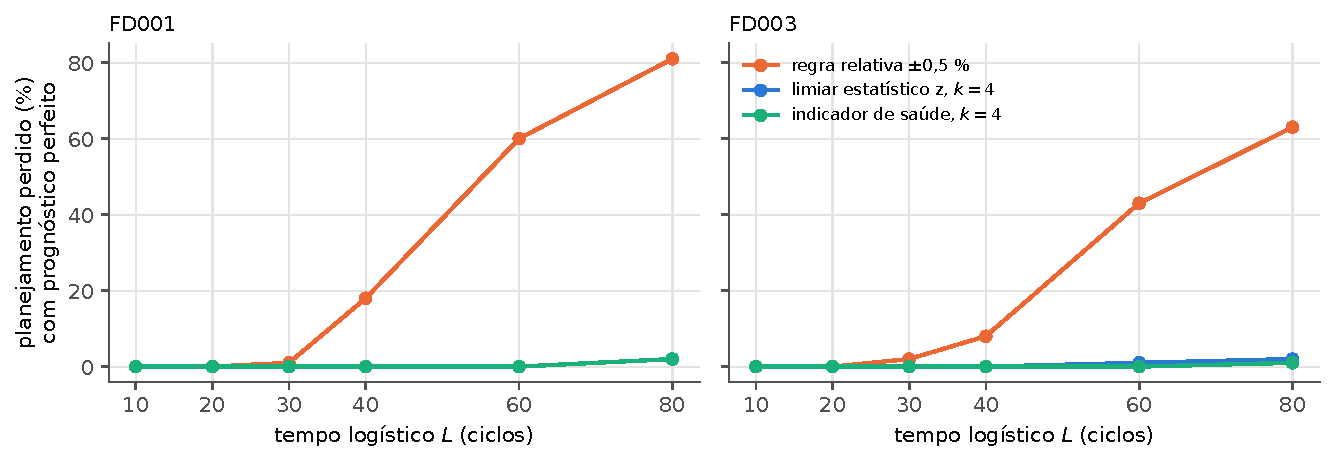
\includegraphics[width=0.92\textwidth]{limite_deteccao}
  \vfill
  \small
  \begin{tabular}{@{}lccc@{}}
    \toprule
    Detector (FD001) & Ciclos P--F: mediana & Mínimo & P em \% da vida \\
    \midrule
    Regra relativa $\pm 0{,}5\,\%$ & 54 & 22 & 71\,\% \\
    Limiar estatístico, $k = 4$ & 140 & 71 & 30\,\% \\
    Indicador de saúde, $k = 4$ & 134 & 69 & 33\,\% \\
    \bottomrule
  \end{tabular}
\end{frame}

\begin{frame}{Onde está a perda?}
  Com detectores de limiar estatístico:
  \begin{itemize}
    \item \textbf{até $L = 60$ ciclos}, a detecção tardia não causa nenhum planejamento perdido no FD001; quase toda a perda (1–3\,\% dos motores) vem do \textbf{erro do prognóstico};
    \item em $L = 80$, a detecção começa a pesar (1–6 pontos percentuais).
  \end{itemize}
  \medskip
  Com a regra relativa de $\pm 0{,}5\,\%$:
  \begin{itemize}
    \item mesmo um prognóstico perfeito perderia o planejamento em \textbf{18\,\%} dos motores com $L = 40$ e em \textbf{60\,\%} com $L = 60$.
  \end{itemize}
  \vfill
  \begin{alertblock}{Lição}
    Antes de investir em modelos de RUL mais precisos, verifique se o \textbf{critério de detecção} deixa janela suficiente para o tempo logístico da sua operação.
  \end{alertblock}
\end{frame}

\begin{frame}{Vida desperdiçada}
  \centering
  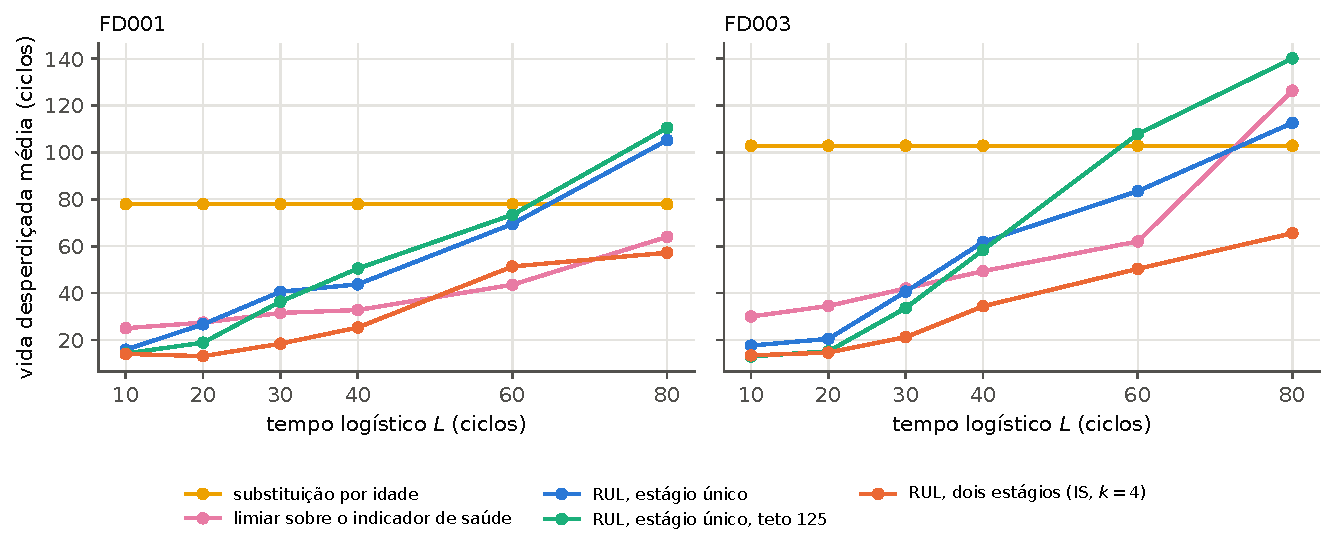
\includegraphics[width=0.95\textwidth]{politicas_desperdicio}
  \vfill
  \small O método em dois estágios reduz a vida desperdiçada quase pela metade para $L \geq 30$ (FD001, $L = 40$: 25 contra 44–51 ciclos). Em contrapartida, aumenta um pouco a proporção de motores cuja remoção chega tarde.
\end{frame}

\begin{frame}{Custo por ciclo voado}
  \centering
  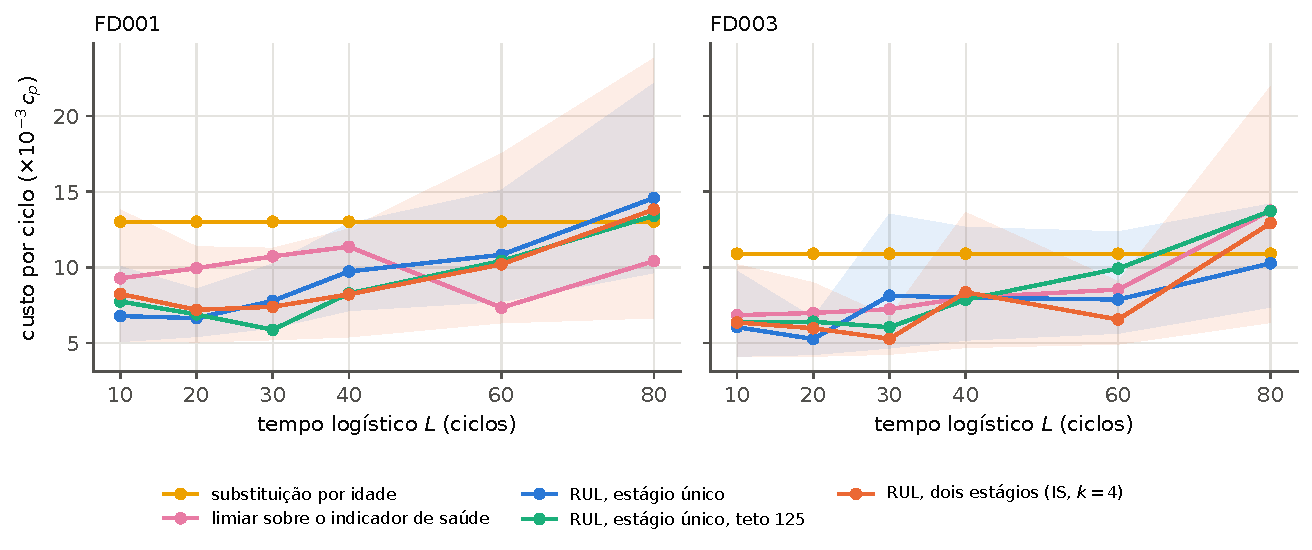
\includegraphics[width=0.90\textwidth]{politicas_custo}
  \vfill
  \small Faixas: intervalos de confiança (IC) de 95\,\%. Os dados ainda não permitem concluir que uma política com sensores tem custo menor que outra. Isso inclui o indicador de saúde, que não usa RUL. Com 100 motores e falhas raras, é difícil detectar diferenças pequenas.
\end{frame}

\begin{frame}{Uma margem maior: o que ganhamos e o que antecipamos?}
  \small
  No estudo de Amanda, aumentar o quantil amplia a margem subtraída da previsão.
  \par\medskip
  \centering
  \begin{tabular}{@{}lccc@{}}
    \toprule
    Quantil & Margem & Previsões & Tardias na faixa \\
            & (ciclos) & tardias & ``manutenção requerida'' \\
    \midrule
    0,75 & 5,34 & 6 & 2 \\
    0,80 & 6,56 & 5 & 2 \\
    0,95 & 16,64 & 0 & 0 \\
    \bottomrule
  \end{tabular}
  \par\medskip
  \raggedright
  \begin{itemize}
    \item A margem maior reduz as previsões tardias observadas neste teste.
    \item Ela também antecipa recomendações. Para escolher, precisamos de \textbf{vida aproveitada, custo e tempo logístico}.
  \end{itemize}
  \textbf{Discussão:} zero previsões tardias basta para escolher a melhor política?
  \fonte{Bassani (2026), slide 28: FD001, CatBoost, 100 motores de teste. Faixa ``manutenção requerida'': menos de 15 ciclos na classificação da defesa.}
  \note{A tabela reproduz três linhas do estudo de Amanda. A coluna Accuracy foi omitida porque sua definição formal não aparece no slide fonte. As faixas de ação daquele estudo são escolhas ilustrativas. Zero previsões tardias no teste é um resultado amostral e não demonstra zero falhas durante o acompanhamento sequencial. Retome a diferença entre avaliar previsões e avaliar uma política de remoção com L ciclos de antecedência.}
\end{frame}

\begin{frame}{O que aprendemos até aqui}
  \begin{enumerate}
    \item Nos cenários avaliados, remover por idade desperdiça cerca de 80–100 ciclos por motor, mais que as políticas com sensores.
    \item O \textbf{critério de detecção do ponto P} determina até que antecedência é possível planejar. Limiares relativos ao nível do sinal encurtam a janela P--F de cerca de 140 para 54 ciclos.
    \item Com detecção estatística, a perda de planejamento vem quase toda do \textbf{erro do prognóstico} para $L \leq 60$.
    \item O método em dois estágios reduz a vida desperdiçada; os dados ainda não demonstram redução de custo frente às outras políticas com sensores.
    \item O custo em motores novos supera o estimado durante a escolha das configurações: 1,8--1,9 vez, contra 1,3--1,4 nas políticas mais simples. Essa avaliação favorável na seleção é chamada de \textbf{otimismo de seleção}.
  \end{enumerate}
\end{frame}

%=====================================================================
\section{Limitações e próximos passos}

\begin{frame}{Limitações do experimento apresentado na aula}
  \begin{columns}[T]
    \begin{column}{0.48\textwidth}
      \textbf{Limitações}
      \begin{itemize}
        \item Os resultados vêm de dados simulados; a aplicação real exige validação própria.
        \item Os arquivos não informam o início físico da degradação.
        \item Tempos logísticos e custos foram escolhidos para os cenários, sem dados de um operador.
        \item 100 motores por subconjunto: intervalos de confiança largos.
      \end{itemize}
    \end{column}
    \begin{column}{0.48\textwidth}
      \textbf{Próximos passos}
      \begin{itemize}
        \item Ajustar o detector considerando alarmes sem degradação relevante.
        \item Escolher a margem para limitar a proporção de remoções tardias.
        \item Treinar no FD001 e avaliar no FD003, que acrescenta degradação do fan.
        \item Avaliar FD002/FD004: 509 motores de treino e seis condições operacionais.
      \end{itemize}
    \end{column}
  \end{columns}
\end{frame}

\begin{frame}{Questões para discussão}
  \begin{enumerate}
    \item Na sua organização, qual é o tempo logístico $L$ para remover um motor? Ele cabe na janela P--F que os dados permitem detectar?
    \item Como estimar $c_f/c_p$ incluindo indisponibilidade da aeronave e risco à segurança? AOG (\emph{Aircraft on Ground}) é a aeronave parada em solo por um impedimento à operação.
    \item Uma detecção ``cedo demais'' tem custo? Em que arquitetura ela passa a ter?
    \item Por que um erro de previsão menor não garante uma decisão melhor? RMSE é a raiz da média dos erros ao quadrado: uma medida de erro na unidade da RUL.
    \item O que mudaria com uma frota real: manutenções intermediárias, trocas de módulo, ruído de medição?
  \end{enumerate}
\end{frame}

\begin{frame}{Referências}
  \scriptsize
  \begin{itemize}
    \item Saxena, A.; Goebel, K.; Simon, D.; Eklund, N. Damage propagation modeling for aircraft engine run-to-failure simulation. \emph{Proc.\ Int.\ Conf.\ Prognostics and Health Management}, 2008.
    \item Bassani, A. S. \emph{An explainable data-driven framework for aircraft engine remaining useful life prediction and maintenance decision support}. Apresentação de defesa de mestrado, ITA, 5 out. 2026.
    \item Saxena, A. et al. Metrics for offline evaluation of prognostic performance. \emph{Int.\ J.\ Prognostics and Health Management} 1(1), 2010.
    \item Wang, W. An overview of the recent advances in delay-time-based maintenance modelling. \emph{Reliab.\ Eng.\ Syst.\ Saf.} 106:165--178, 2012.
    \item Nguyen, K.T.P.; Medjaher, K. A new dynamic predictive maintenance framework using deep learning for failure prognostics. \emph{Reliab.\ Eng.\ Syst.\ Saf.} 188:251--262, 2019.
    \item de Pater, I.; Reijns, A.; Mitici, M. Alarm-based predictive maintenance scheduling for aircraft engines with imperfect remaining useful life prognostics. \emph{Reliab.\ Eng.\ Syst.\ Saf.} 221:108341, 2022.
    \item Mitici, M.; de Pater, I.; Barros, A.; Zeng, Z. Dynamic predictive maintenance for multiple components using data-driven probabilistic RUL prognostics: the case of turbofan engines. \emph{Reliab.\ Eng.\ Syst.\ Saf.} 234:109199, 2023.
    \item Kamariotis, A. et al. A metric for assessing and optimizing data-driven prognostic algorithms for predictive maintenance. \emph{Reliab.\ Eng.\ Syst.\ Saf.} 242:109723, 2024.
  \end{itemize}
\end{frame}

\begin{frame}{Amanda: limitações e propostas de pesquisa futura}
  \begin{columns}[T]
    \begin{column}{0.47\textwidth}
      \textbf{Limitações declaradas}
      \begin{itemize}
        \item Avaliação apenas em FD001 e FD003.
        \item Uma condição operacional por conjunto.
        \item Validação com dados simulados.
        \item Hiperparâmetros (configurações dos modelos) sem otimização.
        \item Limiares fixos para recomendar manutenção.
      \end{itemize}
    \end{column}
    \begin{column}{0.49\textwidth}
      \textbf{Pesquisas propostas}
      \begin{itemize}
        \item Incluir FD002 e FD004: operação em condições variadas.
        \item Validar com dados de frotas reais.
        \item Desenvolver limiares que se adaptem aos dados.
        \item Otimizar a manutenção considerando custos.
        \item Explicar as previsões para apoiar processos de certificação.
      \end{itemize}
    \end{column}
  \end{columns}
  \fonte{Fonte: Amanda Schneider Bassani (2026), slide 38 da defesa. A tarefa usa apenas FD001 para iniciar a investigação da decisão de manutenção.}
  \note{Estas são as limitações e propostas declaradas por Amanda, distintas das limitações do experimento de LightGBM apresentado na aula. Hiperparâmetros são configurações escolhidas antes de treinar o modelo. Explicabilidade orientada à certificação é uma proposta de pesquisa, não uma certificação já obtida. Convide cada aluno a identificar uma pergunta pequena que consiga testar no FD001.}
\end{frame}

\end{document}
